% \begin{figure}[!t]
%     \centering
%     \includegraphics[width=\linewidth]{images/example.png}
%     \caption{A proposed planning framework.}
%     \label{fig:flowchart}
% \end{figure}

\begin{figure}
\centering
\captionsetup[subfigure]{width=\linewidth}
\subfloat[subfig:plans][Recommendations from some planner. 
Here a `$+$' represents an \textit{increase}, a `$-$'   and a `$\cdot$' represents \textit{no-change}.]{
\resizebox{0.8\linewidth}{!}{
\begin{tabular}{ccccccccc}
\hline
\rowcolor{Gray} DIT & NOC & CBO & RFC & FOUT & WMC & NOM & LOC & LCOM \\
$\cdot$ & $\cdot$    & $\cdot$    & $+$   & $\cdot$     & $+$   & $+$   & $+$   & $+$    \\\hline
\end{tabular}}
\label{subfig:plans}
}\\

\subfloat[][A sample of possible actions developers can take.
 Here a `$+$' represents an \textit{increase}, a `$-$' represents a \textit{decrease}, and an empty cell represents \textit{no-change}.
Taken from~\cite{stroggylos2007, du2006study, kataoka2002, bryton2009,elish2011,elish2012}. The action highlighted in \colorbox{lightgray}{gray} shows an  action matching XTREE's   recommendation.]{
\resizebox{\linewidth}{!}{
\begin{tabular}{lccccccccc}
\hline
\rowcolor{Gray}Action                                      & DIT & NOC & CBO & RFC & FOUT & WMC & NOM & LOC & LCOM \\ 
Extract Class                               &     &     & $+$   & $-$   & $+$    & $-$   & $-$   & $-$   & $-$    \\
\rowcolor{lightgray} Extract Method                              &     &     &     & $+$   &      & $+$   & $+$   & $+$   & $+$    \\
Hide Method                                 &     &     &     &     &      &     &     &     &      \\
Inline Method                               &     &     &     & $-$   &      & $-$   & $-$   & $-$   & $-$    \\
Inline Temp                                 &     &     &     &     &      &     &     & $-$   &      \\
Remove Setting Method                       &     &     &     & $-$   &      & $-$   & $-$   & $-$   & $-$    \\
Replace Assignment                          &     &     &     &     &      &     &     & $-$   &      \\
Replace Magic Number                        &     &     &     &     &      &     &     & $+$   &      \\
Consolidate Conditional                     &     &     &     & $+$   &      & $+$   & $+$   & $-$   & $+$    \\
Reverse Conditional                         &     &     &     &     &      &     &     &     &      \\
Encapsulate Field                           &     &     &     &     &      & $+$   & $+$   & $+$   & $+$    \\
Inline Class                                &     &     & $-$   & $+$   & $-$    & $+$   & $+$   & $+$   & $+$    \\ \hline
\end{tabular}}
\label{subfig:actions}
}\\
\subfloat[Before `extract method'][Before `extract method']{
\fbox{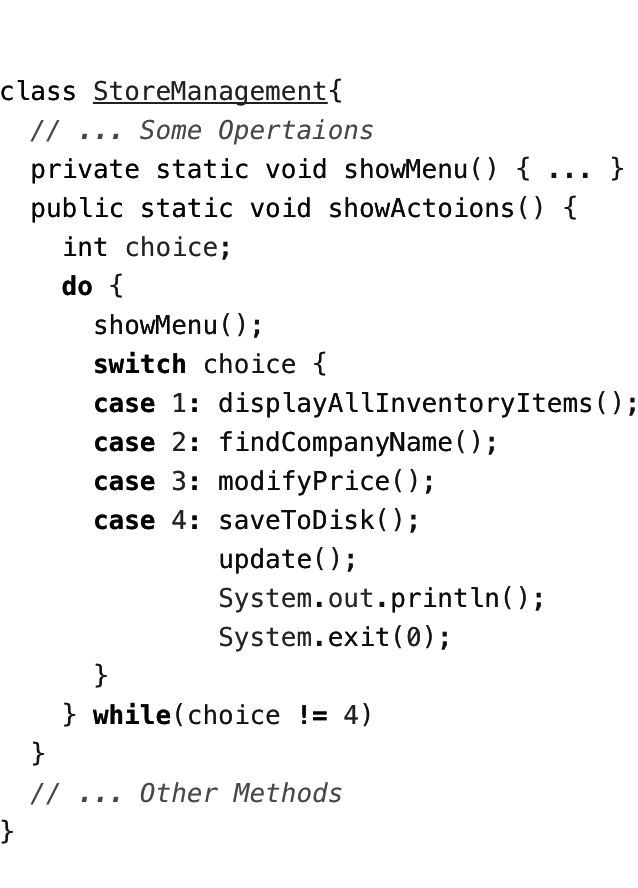
\includegraphics[width=0.45\linewidth]{1.png}}
\label{subfig:before}
}
\subfloat[After `extract method'][After `extract method']{
\fbox{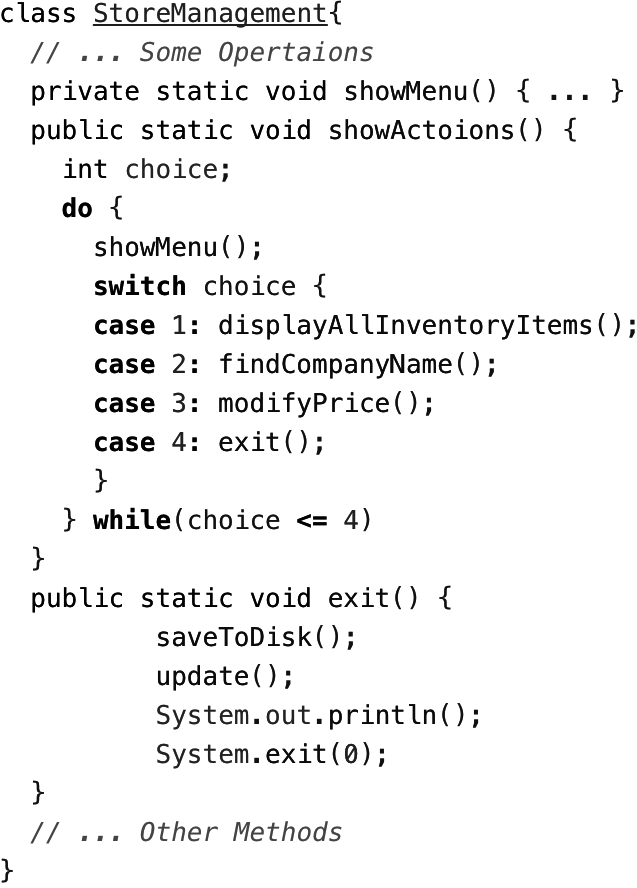
\includegraphics[width=0.45\linewidth]{2.png}}
\label{subfig:after}
}

\caption{An example of how developers might use XTREE to reduce software defects.}
\label{fig:motivating_example}
\end{figure}